\chapter{FC-CMOS gates}

\section{Sizing of single transistor inside a logic gate}
Once the transistor are placed in order to compute the requested logic function the sizing of the single transistor has to follow this simple rule: the equivalent resistance in the worst case state has to be equal to the one of an inverter of the same size of the gate.\\
Transistor in parallel show a resistance half of a single transistor so considering the following NAND gate with a size equal to 1 the p-mos will have an aspect ratio of 3 and the n-mos of 2 (two transistor of size 2 in series are the equivalent of a transistor of size 1).\\

\centering
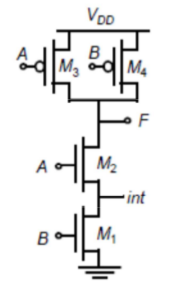
\includegraphics[width=0.15\textwidth]{C6_1.png}\\
\raggedright

If the searched size was s=2 we will have p-mos 6 and n-mos 4 of aspect ratio.\\

\section{Equivalent capacitance}
To estimate the equivalent internal capacitance $C_{int}$ of a generic FC-CMOS gate we have to look to the dimesnions of the transistors connected to the output node. The sum of the aspect ratios of this transistors divided by 4 it's how many $C_g^{(0)}$ the internal capacitance is.\\
\vspace{5mm}
To better assest the propagation delay we should also take into account the inter-nodes capacitance inside our gate; this leads us to a more complex analysis since we have to consider whitch parasitic capacitance are charged an whitch are discharged and we shoulde use the Elmore theorem for every transistion.

\centering
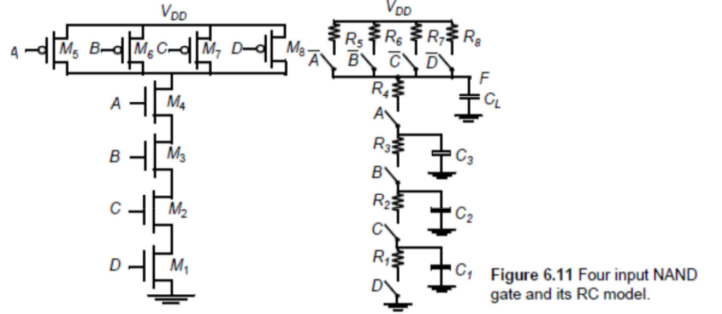
\includegraphics[width=0.5\textwidth]{C6_2.png}\\
\raggedright

This inter-nodes capacitance can't be estimated as before with a value of 2fF but , since 2 transistor in series are integrated with common drain-source, with 1fF capacitance.\\


\centering
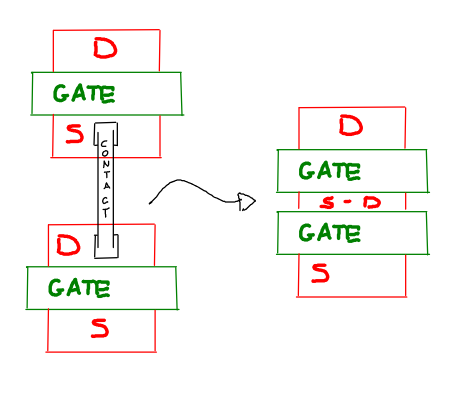
\includegraphics[width=0.35\textwidth]{C6_3.png}\\
\raggedright

We can neglect the effect of the inter-nodes capacitance since our gates have small fan-in (3-4 max).\\

\vspace{5mm}
In case of large fan-in and a lot of transistors in series it's possible to adopt clever sizing "inspired" by the inverter chain optimization 

\centering
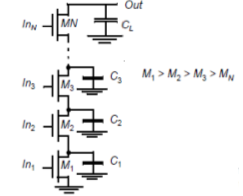
\includegraphics[width=0.35\textwidth]{C6_4.png}\\
\raggedright

\vspace{5mm}
Another good rule of thumb is that the last signal coming to the gate (the slowest signal at the input of the gate) has to be connected to the transistor closest to the output.\\

\section{Propagation delay}

\subsection{Equivalent resistance}
We define the equivalent resistance of a generic gate of size s (built with the right internal proportion described before) as 
\begin{equation}
R_{eq}=\frac{R_{eq}^{(1)}}{s}=\frac{11.6k\Omega}{s}
\end{equation}

\subsection{"p" factor}
The factor "p" or intrinsic delay factor (OUTPUT) it's a constant that connect the intrinsic capacitance of our gate with the intrinsic capacitance of an inverter of the same dimensions and can be calculated as 
\begin{equation}
p=\frac{C_{int}(s=1)}{C_{int}^{(1)}}
\end{equation}
\begin{equation}
p=\frac{\sum \frac{W}{L}|_{mos \ connected \ to \ y}}{4*s}
\end{equation}
and it's releted with the intrinsic capacitance of a generic size gate as 
\begin{equation}
C_{int}=spC_{int}^{(1)}
\end{equation}
This parameter it's indipendent on the size of the gate

\subsection{"g" factor}
The factor "g" is the logical effort (INPUT) that quantifies the complexity of the gate with respect to the inverter in the "input" direction.\\
Also this parameter is indipendent on size and has to be calculated considering single couple of inputs\\ 
\begin{equation}
g=p=\frac{C_{g}(s=1)}{C_{g}^{(1)}}
\end{equation}
\begin{equation}
g=\frac{\sum \frac{W}{L}|_{mos \ connected \ to \ A}}{4*s}
\end{equation}


\vspace{6mm}
\centering
Here some examples of this parameters on famous logic gates\\
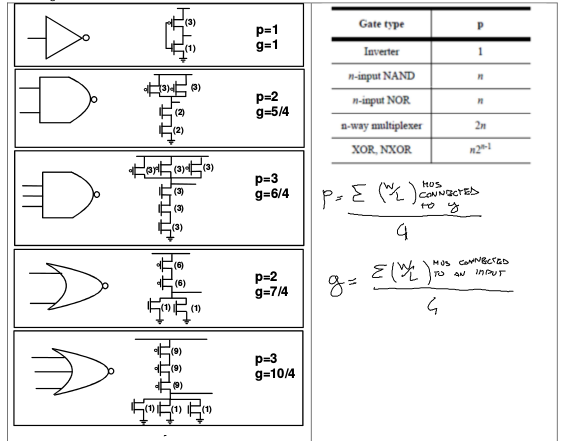
\includegraphics[width=0.75\textwidth]{C6_5.png}\\
\raggedright

\subsection{Propagation delay}
The expression of the propagation delay of a generic gate is
\begin{equation}
\tau_p=\tau_{p0}\left(p+\frac{fg}{\gamma}\right)
\end{equation}
where we can distinguish two contributions; the term $\tau_{p0}$ is the intrinsic delay and $fg\tau_{p0}$  is the effort delay strictly related to the load capacitance. The product fg it's called stage effort or h.\\

\section{Size optimization of $\tau_p$}
The delay that counts and that we are going to optimize it the one related with the critical path, the delay of the longest path.\\
To optimize the propagation delay we need that all the gates have the same stage effort h.\\
\vspace{5mm}
We define the path fan-out as 
\begin{equation}
F=\frac{C_L}{C_{g,1}}
\end{equation}
and the path logical effort as 
\begin{equation}
G=\prod g_i
\end{equation}
To optimize the propagation delay we all the stages has to have the following $h_{opt}$
\begin{equation}
h_{opt}=\sqrt[N]{H}
\end{equation}
This corresponds to a propagation delay of the overall chain of 
\begin{equation}
\tau_{p,opt}=\tau_{p0}\left( (\sum p)+\frac{N h_{opt}}{\gamma} \right)
\end{equation}
in this way the dimension of the j-th stage will be 
\begin{equation}
s_j=\frac{s_1g_1}{g_j}\prod_{i=1}^{j-1}f_i
\end{equation}


























